% style notes
% - \,percent not \%

\documentclass[12pt, preprint]{aastex}
\usepackage{bm, graphicx, subfigure, amsmath, morefloats}

% words
\newcommand{\project}[1]{\textsl{#1}}
\newcommand{\thecannon}{\project{The~Cannon}} 
\newcommand{\tc}{\project{The~Cannon}} 
\newcommand{\apogee}{\project{APOGEE}}
\newcommand{\apokasc}{\project{APOKASC}}
\newcommand{\aspcap}{\project{ASPCAP}}
\newcommand{\corot}{\project{Corot}}
\newcommand{\kepler}{\project{Kepler}}
\newcommand{\gaia}{\project{Gaia}}
\newcommand{\gaiaeso}{\project{Gaia--ESO}}
\newcommand{\galah}{\project{GALAH}}
\newcommand{\most}{\project{MOST}}
\newcommand{\code}[1]{\texttt{#1}}
\newcommand{\documentname}{\textsl{Article}}

\newcommand{\teff}{\mbox{$\rm T_{eff}$}}
\newcommand{\kms}{\mbox{$\rm kms^{-1}$}}
\newcommand{\feh}{\mbox{$\rm [Fe/H]$}}
\newcommand{\xfe}{\mbox{$\rm [X/Fe]$}}
\newcommand{\alphafe}{\mbox{$\rm [\alpha/Fe]$}}
\newcommand{\mh}{\mbox{$\rm [M/H]$}}
\newcommand{\logg}{\mbox{$\rm \log g$}}
\newcommand{\noise}{\sigma_{n\lambda}}
\newcommand{\scatter}{s_{\lambda}}
\newcommand{\pix}{\mathrm{pix}}
\newcommand{\rfn}{\mathrm{ref}}
\newcommand{\rgc}{\mbox{$\rm R_{GC}$}}
\newcommand{\vgal}{\mbox{$\rm V_{GAL}$}}

% math and symbol macros
\newcommand{\set}[1]{\bm{#1}}
\newcommand{\starlabel}{\ell}
\newcommand{\starlabelvec}{\set{\starlabel}}
\newcommand{\mean}[1]{\overline{#1}}
\newcommand{\given}{\,|\,}
%\newcommand{\teff}{\mbox{$\rm T_{eff}$}}
%\newcommand{\kms}{\mbox{$\rm kms^{-1}$}}
%\newcommand{\feh}{\mbox{$\rm [Fe/H]$}}
%\newcommand{\xfe}{\mbox{$\rm [X/Fe]$}}
%\newcommand{\alphafe}{\mbox{$\rm [\alpha/Fe]$}}
%\newcommand{\mh}{\mbox{$\rm [M/H]$}}
%\newcommand{\logg}{\mbox{$\rm \log g$}}
%\newcommand{\noise}{\sigma_{n\lambda}}
%\newcommand{\scatter}{s_{\lambda}}

% math
\newcommand{\numax}{$\nu_{\max}$}
\newcommand{\deltanu}{$\Delta\nu$}
\bibliographystyle{apj}

\begin{document}



% To do. 
% 1. release two catalogues :
% 1a) trained on log mass and 1b) trained on log mass
%2. resample the errors in label space - add a random error to the mass term and rerun the labels through the cannon and see if the standard deviation and bias in the take one out test is any different - if not we know the noisiness in the training set is not an issue
%3. cut out a lot of regions except for the CN and retrain and see if the take-out-out test sigma increases or decreases in the dispersion - if increases we know we are limited by the information available in the data. If decreases there is degeneracy / noisiness in the covariance of labels? 

% plotting in /Apogee_ages/makeplot_scatter_test18_step.py 
% and plotelements_on_spectra.py 

\title{Measuring red-giant masses and ages with stellar spectra: An age catalogue of the Milky Way disk from \apogee }
\author{M.~Ness\altaffilmark{1},
David~W.~Hogg\altaffilmark{1,2,3},
H.-W.~Rix\altaffilmark{1},
M.~Martig \altaffilmark{1},
\textbf{others}}
\altaffiltext{1}{Max-Planck-Institut f\"ur Astronomie, K\"onigstuhl 17, D-69117 Heidelberg, Germany}
\altaffiltext{2}{Center for Cosmology and Particle Physics, Department of Phyics,
             New York University, 4 Washington Pl., room 424, New York, NY, 10003, USA}
\altaffiltext{3}{Center for Data Science, New York University, 726 Broadway, 7th Floor, New York, NY 10003, USA}
% \altaffiltext{4}{NSF Astronomy and Astrophysics Postdoctoral Fellow}
% \altaffiltext{5}{Department of Physics \& Astronomy, Johns Hopkins University, Baltimore, MD, 21218, USA}
\email{ness@mpia.de}

\begin{abstract}%
% Context
With \thecannon, we have demonstrated that it is possible to use a
small training set of stars with noisy spectral data and known
stellar-parameter labels to build a data-driven probabilistic model of
stellar spectra that can be used to infer stellar-parameter labels for
other stars (with differently noisy spectral data).
% Aims
% Method
Here we train this system using stars with known stellar mass labels
obtained from a training set of stars with both
\kepler\ asteroseismological observations (with derived masses) and
\apogee\ infrared spectral data.
We find that after training on mass, \thecannon\ can infer stellar
masses---and therefore also stellar ages---for red-giant stars using
infrared spectral data alone. \tc\ returns (log) masses to an accuracy of 0.08~dex and (log) ages to 0.25 dex for typical-quality \apogee\ spectra.  We produce a catalogue of mass and inferred age labels for all XXX,000 red-giant stars in \apogee\ DR12 and investigate the age distribution in the Milky Way's disk using the red clump sample of 20,000 stars, which span a galactic radius of 4 - 14 kpc and which have small distance errors ($\approx$ 5\, percent). We show from these data that the ages of stellar structures in the Milky Way demonstrate an evolution consistent with inside out formation and radial mixing for longer lived stars, even conditioned on abundances. We demonstrate that the capability to infer age from spectroscopy alone works mathematically using cross validation and we show that the mass information derives from elements associated with dredge-up processes predicted by stellar evolution. This capability opens up new opportunities for Milky Way and stellar astrophysics.

% Results
%We demonstrate the validity of the stellar masses and ages that we determine with \tc\ with three
%methods:
%Cross-validation demonstrates that the method obtains (log) mass accuracies of approximately 0.08~dex and (log) age accuracies
%of roughly 0.25~dex for typical-quality \apogee\ spectra.
%We find that the spectral mass (or age) indicators
%discovered by \thecannon\ are associated with elements that can be ``dredged up'',
%specifically, the CN regions of the spectra. We produce a catalogue of mass and inferred age labels for all XXX,000 red-giant stars in \apogee\ DR12 and investigate and age distribution in the Milky Way's disk using the \apogee\ red clump sample in particular, which spans a galactic radius of 4 - 14 kpc and which have small distance errors ($\approx$ 5\, percent). We show from this that the ages of stellar structures in the Milky Way follow evolution consistent with inside out formation and radial mixing processes that are relevant for longer lived stars, even conditioned on abundances.
%All three of these tests show that we can obtain red-giant mass and
%age information from stellar spectra; these capabilities open up new
%opportunities for Milky Way and stellar astrophysics. 

\end{abstract}

\keywords{%
keywords: incomplete (DWH)!
---
methods: data analysis
---
methods: statistical
---
stars: abundances
---
stars: fundamental parameters
---
surveys
---
techniques: spectroscopic
}

\section{Introduction}\label{sec:Intro}

Asteroseismology surveys, such as \most, \corot, and \kepler, have
been extremely successful and productive in bringing us information
about stellar interiors and (therefore) ages.
These missions operate by taking high-cadence, high-precision stellar
photometry, in which stellar oscillation modes are visible in the
Fourier domain.
These missions have operated by taking long stretches of
uninterrupted, uniform, dense imaging data on thousands of individual
stars.
They are expensive missions, but absolutely critical to calibrate
physical stellar interior models and set standards for stellar
parameter estimation, all of which is required for the ultimate
success of the next generation of stellar surveys, particularly
including the \gaia\ Mission.

At the same time, there are many large spectroscopic surveys, such
as \apogee\ \citep{Majewski2012}, \gaiaeso\ \citep{Gilmore2012} and \galah\ \citep{Freeman2012}, underway to measure the properties
of stellar \emph{exteriors}.
These surveys will take high signal-to-noise, high resolution spectra
of hundreds of thousands of stars, revealing detailed surface chemical
abundances.
One question that naturally arises is:
How do we use these two pieces of information of surface spectroscopy
and interior asteroseismology to jointly infer stellar properties?
Another is:
Is there any way we could learn about stellar interiors from surface
spectroscopy?
After all, the marginal cost of taking a spectrum of
a new star is very low relative to the marginal cost of getting its
asteroseismology.

Using astroseismology, stellar mass is determined for stars directly from the scaling relations which describe the frequency spacing and amplitude of the modes as a function of the mass. For inferring mass and therefore age information from surface spectroscopy alone, there are only a small handful of specific metrics in the optical and UV wavelength bands that have been previously used  \citep[see][and references therein]{soderblom2010}. These metrics derive from rotation, in the line-profile variations due to non-LTE effects (as convection scales with mass) and from chromospheric emission from a time-dependent magnetic field e.g. the Ca II HK and H$\alpha$ features. The decay of long lived isotopes such as Th, which can be measured at 4019 Angstroms, can also be used for age dating by comparing the abundance of the long lived isotopes to that of the stable elements in the stellar photosphere. 


Typically, age estimates have been determined for main sequence and turn-off stars not from spectral features themselves, but from using the measured stellar parameters by interpolating between stellar models. In the main-sequence and turn-off \teff-\logg\ regime, the stellar evolution models are the least insensitive to age. The stellar parameters are typically derived from high resolution spectroscopy, which delivers low associated errors on the parameters) \citep[e.g.][]{Bensby2013, Casagrande2011, haywood2013}.   However, the age constraints obtained using this method are typically weak or may only provide an upper limit on the estimated age.  This approach has been used to determine ages for what has been up until now the largest homogeneous data set of stellar ages in the galactic disk, from the Geneva Cophenhagen Survey (GCS). All of the 16,682 main sequence stars from GCS are located in the solar neighbourhood \citep{nordstrom2004short}.

If we can instead determine the interior properties of stars from surface
spectroscopy alone, even noisily, great opportunities arise for
studying the stellar populations of the Milky Way and their formation. 

In general, mass and therefore inferred age might only appear in the spectra as
certain combinations of surface abundances that are highly covariant
with age.  For example, older stars in the Milky Way tend to be more
alpha-enhanced.  We will consider such age indicators illegitimate;
the purpose of this project is to obtain estimates for ages and masses \emph{that work even within narrow abundance-selected subsamples}.


We use \tc\  \citep{Ness2015} to infer stellar mass, \teff, \logg, \feh\ and \alphafe\ for \apogee\ stars.  Our data-driven generative model quantifies the information content at each pixel. Therefore, we are able to examine the origin of the information in the spectra for our five labels of \teff, \logg, \feh, \alphafe\ and mass. We have shown previously, in  \citet{Ness2015},  that \tc\ is successful for delivering the three primary labels of \teff, \logg\ and \feh\ for \apogee\ stars. The additional mass label (and \alphafe\ label) that we infer in this work is able to be determined because we have a training set of stars, which have known masses (and very accurate \logg\ labels) from astroseismology and known stellar parameters of \teff, \feh\ and \alphafe\ from \apogee's stellar pipeline \aspcap. We deliver our catalogue of mass and inferred ages for the 20,000 red clump stars in the \apogee\ survey, which have well known distances, as well as for the XXXX giant stars in the DR12 \apogee\ data release.


%The red clump sample alone from \apogee\ in itself, for which accurate distances (to 5 percent) have been determined, comprises 20,000 stars \citep{Bovy2014} and spans a radial extent across the disk of 6 -- 14 kpc. 

%We show that the spectroscopic  information informing the masses and other labels, as identified by \tc\ is in line with expectations of chemical evolution and stellar physics and we demonstrate that the mass and inferred age labels that are determined provide an additional dimension of information (that is, our age measurement does not reflect a proxy for alpha/Fe). 

%, with a sample of about 16,682 stars, has been the largest sample of stars, all of which are nearby main sequence stars, with complete data on stellar ages in the Milky Way disk. These ages have been determined from the constraints set by the measured parallaxes to these stars and their stellar parameters of \teff, \logg\ and \feh,  using interpolation between stellar isochrone models \citet{Holm2009}.



%We similarly use stellar models but determine our mass directly from the spectra - and use the models to move from measured inferred mass to inferred age. Not mapping from stellar params to isochrone age space. How do I say this in a better way to describe why it is better? 



%Skumanich 1972 - empirical age estimators - Rotation (less relevant once giant) and chromospheric emission - Ca II HK and H-alpha (Magnetic fields manifested as activity) . 

%mention in paper - training set currently small - catalogue of 8K APOKASC stars is coming \\. 

%\ldots DWH: What are our hypotheses about how mass or age might appear
%in a stellar spectrum?  It might appear as dredge-up of evolved
%material from the core into the photosphere.  It might appear as
%chromospheric emission from a time-dependent magnetic field.  It might
%appear as line-shape variations as stellar rotation evolves.  It might
%appear as amplitude variations in non-LTE effects as convection scales
%are different for stars of different masses.

%\ldots DWH: Importantly, age might only appear in the spectra as
%certain combinations of surface abundances that are highly covariant
%with age.  For example, older stars in the Milky Way tend to be more
%alpha-enhanced.  We will consider such age indicators illegitimate;
%the purpose of this project is to obtain estimates for ages and masses
%\emph{that work even within narrow abundance-selected subsamples}.

\section{Methods and data}

We make use of \tc\ \citep{Ness2015}, which is a data-driven method for
determining stellar parameters and abundances.
\tc\ is a probabilistic model of stellar spectra---meaning that it
produces a likelihood function or a probability density in spectral
space---that is itself a function of stellar parameters and chemical
abundances (which we collectively call ``labels'').
The model is not based on physical models, but is instead learned
from a training set of stars with (assumed) known labels.
This learning is called the ``training step''.
The model is used to label a new star \emph{not} in the training set,
by maximizing the likelihood of the label values given the new star's
spectrum.
This labeling is called the ``test step''.
\tc\ differs from other kinds of standard machine-learning methods
(such as random forest or deep neural networks) in that it contains an
explicit likelihood function, at both the training step and the test
step, so it is able to account for heteroskedastic noise and missing
data in the spectra of both the training and test stars.

Generally, we take a spectral model to be characterized by a coefficient vector $\set{\theta}_\lambda$
that allows to predict the flux at every pixel $f_{n\lambda}$ for a given label vector $\starlabelvec_n$:


\begin{eqnarray}
f_{n\lambda} &=&
g(\starlabelvec_n |  \set{\theta}_\lambda) + \mbox{noise}
\label{eq:specmodel}\quad 
\end{eqnarray}

In detail, the likelihood function we use for \tc\ has a
gaussian form at each measured spectral wavelength, with a mean that
is a quadratic function of the labels, and a variance that consists of
an intrinsic variance added to an observational noise variance (from
photon noise and other sources). For our model we use a the quadratic-in-labels form, but with a cubic \logg\ term, which was found empirically to improve the accuracy of the \teff\ label in the cross-validation test by $\approx$ 10\,percent.  This model presumes that the continuum-normalized flux is a polynomial of the stellar labels, as below: 

$f_{n\lambda} =
\set{\theta}_\lambda^T \cdot \starlabelvec_n + \mbox{noise}$, 
but where $\set{\theta}_\lambda$ now contains 22 elements at every pixel. For the case of the five labels $(\teff , \logg , \feh, \alphafe, \mbox{mass})$ the label vector $\starlabelvec_n$
becomes  

\begin{equation}
\begin{split}
\starlabelvec_n \equiv  [1, \teff, \logg, \feh, \alphafe, \mbox{mass}, \teff^2, \\
 \teff\cdot\logg, \teff\cdot\feh, \teff\cdot\alphafe, \teff\cdot \mbox{mass},  \logg^2, \\
  \logg\cdot\feh, \logg\cdot\alphafe, \logg\cdot \mbox{mass}, \feh^2, \\
  \feh\cdot\alphafe, \feh\cdot \mbox{mass}, \alphafe^2, \alphafe\cdot \mbox{mass}, \mbox{mass}^2,  \logg^3]
\end{split}
 \label{eq:quad}
\end{equation}


%MKN: Put in model - is quadratic but with a cubed log g term - from empirical testing. Found that this reduced the error in the labels, most significatnly for the teff label, of 10percent. No significant gain going to higher order in the other terms. \\. 

We have shown in previous work \citep{Ness2015} that \tc\ does a good job
of modeling stellar spectra and delivering stellar parameters and
chemical abundances for stars with spectra taken by the \apogee\ project \citep{Majewski2012}.  \apogee\ is an SDSS \footnote{\url{www.sdss.org}} (Eisenstein et al. 2011) infrared survey of the Milky Way disk, bulge and halo and has provided H-band spectra (1500-1700 nm) of about 150,000 stars in the public data release DR12.  Of this sample, there is a subset of stars that also have been observed by the Kepler satellite, with measurements of ${nu}_max$ and $\Delta_{nu}$, that provide stellar mass estimates for these stars in this particular Kepler field. These stars are the \apokasc\ sample \citep{P2014}. In this project, we are once again using \apogee\ data, and once again
using \tc. 

We work with the continuum-normalized DR12 spectra, and the method of continuum
estimation turns out to be important for performance. We use the aspcapStar files provided by \apogee, but apply our own signal-to-noise invariant continuum normalisation by fitting a low-order polynomial to `true' continuum pixels, as described in \citet{Ness2015}. 
The three labels of \teff, \logg\ and \feh\ delivered with \tc\ were demonstrated in \citet{Ness2015}.  In this work we determine two additional labels, of \alphafe\ label and mass. From the mass, we train on log mass, as we find that the error on mass is linear in log mass (and log age) rather than linear mass and age. We infer age, using stellar evolution models. Our five labels are provided to \tc\ in the training step, and delivered by \tc\ in the test step.

Stellar mass is a parameter that is not usually considered visible in
spectral data; in the training set we are obtaining these stellar mass
parameters via asteroseismology. In particular, the training set is taken from the \apokasc\ sample of
stars observed by \apogee\ \citep{Majewski2012}, the first data release of which was made in \citet{P2014}. 
This sample of stars have high-quality infrared
spectra from \apogee\ and also asterosesmological measurements from the \kepler\ mission.
Specifically, they have \numax\ and \deltanu\ measurements from \kepler, derived from the standard scaling relations \citep[see][and references therein]{P2014} and corresponding spectra in the H-band across 1.5-1.7 $\micron$ at a resolution of R $\sim$ 22,500, as part of the \apogee\ survey. 
The \kepler\ Mission \citep{B2010} took continuous, 30-min cadence (or
higher cadence) photometric observations of more than $10^5$ stars,
providing (at least for giant stars) measurements of the
asteroseismological frequencies and frequency splittings that indicate
stellar interior density structure.
The asteroseismological measurements are used---with stellar
models---to infer stellar masses and thus provide labels.

The training set of stars is a 1639 subset of high quality \apokasc\ stars from \citet{Martig2014}. These stars have been selected by \citet{Martig2014} based on additional quality cuts: only stars with no warning or error in the \aspcap\ \code{FLAG} parameter provided by \apogee\ \citep{Ahn2014}, with no rotation flag set and with errors on the  \deltanu\ and $\nu\_{\mbox{max}}$ less than 10\,percent are included. The \apokasc\ stars comprise a high signal-to-noise (SNR) sample, with an average SNR $\approx$ 330 $\pm$ 155. 
%
%Five labels are used for training of \tc, the \teff, \logg, \feh, \alphafe\ and mass.
 The five training labels adopted are from the \aspcap-corrected \citep{Meszaros2013} values for the \teff, \feh\ and \alphafe\ and the astroseismic value for \logg, as determined from the measured $\nu_{max}$ . The mass label was determined from the  \deltanu\ and $\nu\_{\mbox{max}}$ measurements using the standard seismic scaling relation given in \citet{SilvaA2011,Chaplin2011} and repeated in Equation \ref{scaling}.

\begin{equation} \label{eq:mass}
M= \left( \frac{\nu_{\mathrm{max}}}{\nu_{\mathrm{max,\odot}}}\right)^3\  \left( \frac{\Delta \nu}{\Delta \nu_{\odot}}\right)^{-4} \ \left( \frac{T_{\mathrm{eff}}}{T_{\mathrm{eff,\odot}}}\right)^{1.5} \ .
\end{equation}
\label{scaling}


We adopt  $T_{\mathrm{eff,\odot}}=5777$ K, $\nu_{\mathrm{max,\odot}}=3140\ \mu$Hz, $\Delta \nu_{\odot}=135.03\ \mu$Hz, as per \citet{Martig2014}. The solar values  $\Delta \nu_{\odot}$ and $\nu_{\mathrm{max,\odot}}$ are those used for the \apokasc\ catalogue and were obtained by \cite{Hekker2013}.

To transform the mass label determined by \tc\ to an inferred age label for each star, we use the PARSEC isochrones \citep{Bressan2012} with a mass loss parameter of $\eta_{\mbox{Reimers}}$ = 0.2 and adopt the red clump evolutionary state to set the relationship between mass and age at each metallicity.  The mapping of mass to age is directly tied to the models and subject to assumptions including the models chosen, the stellar mass loss parameter and the evolutionary state. These assumptions lead to small absolute differences in the age scaling of the stars given the mass. However,  the relative ages are consistent and quantatively we draw no different conclusions in any of our results by varying these primary input assumptions. For example, assuming a red clump evolutionary state ( instead of a red giant) does not change the age distribution of the sample and individual stellar age differences are on the order of $<$ 5\,percent between these two evolutionary states. 

\section{Experiments and results}

\subsection{Validation of the mass and age determinations}

To determine the uncertainties on our individual \teff, \logg, \feh, \alphafe\ and mass, we perform a take-stars out test on the set of reference objects.
For the take-stars out test we train the spectral model iteratively on 90\,percent of the reference spectra and then run the test step on the remaining 10\,percent of the spectra and we do this 10 times, stepping through each next 10\,percent of the data. Our results are shown in \figurename~\ref{fig:validation1} for the five labels. The input (x-axis) labels are from \aspcap\ and astroseismology, as described in Section X and the output (y-axis) labels are the output labels are from \tc.  The sixth panel in this Figure shows the masses transformed to ages using interpolation between the PARSEC isochrones, where the red clump evolutionary state has been adopted on the isochrones at each age and \feh. 

This \figurename\ shows that \tc 's purely mathematical approach of label transfer estimates the stellar labels with accuracies of 35K in \teff, 0.08 dex in \logg, 0.02 in \feh, 0.02 in \alphafe\ and  0.08 dex in log mass, or 0.25 dex in log age (Gyr) over the label-range of the reference stars. It is important to remember that the objects plotted are the left-out objects and the spectrum of these objects are completely detached from the training step,  except that they have the same experimental set-up and are drawn from a part of label space that is represented by the remaining reference objects.

%plotdiff_5labels_10percent_linear_orig.py trained on 1639 stars if
%run -i plotdiff_5labels_10percent_linear trained on 1500 stars
%/Users/ness/new_laptop/TheCannon/TheCannon/code/ plotdiff_5labels_10percent_contour.py
%/Users/ness/new_laptop/TheCannon/TheCannon/code/ plotdiff_6labels_10percent_contour.py
\begin{figure}[h!]
\centering
        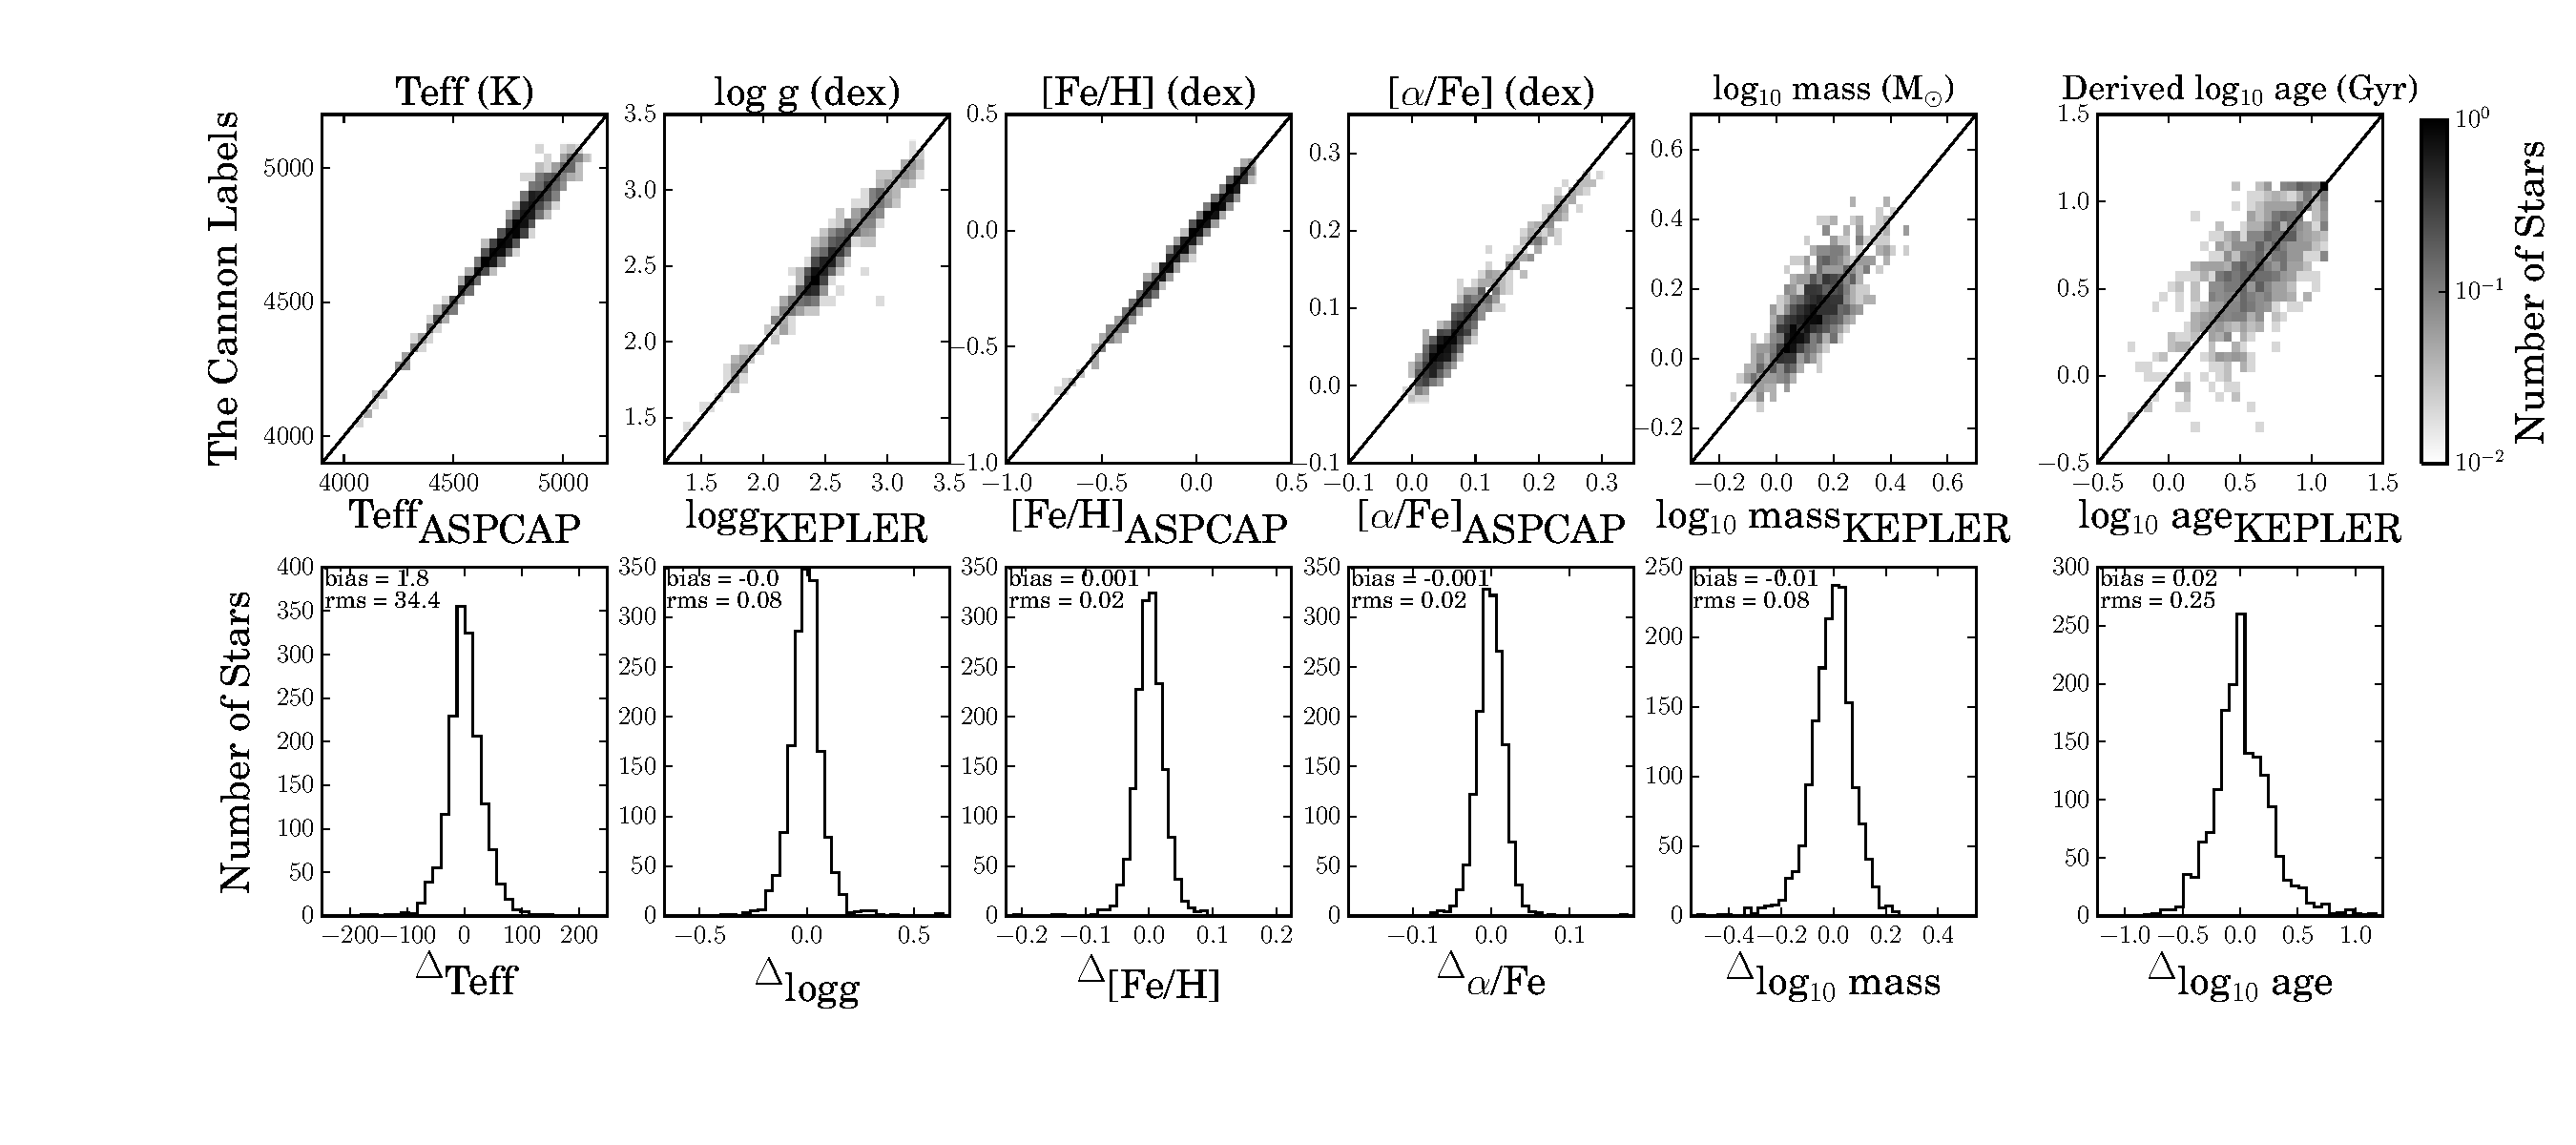
\includegraphics[scale=0.35]{./plots/validation_1639_6.pdf}
  \caption{Cross validation of training dataset of 1639 stars, for the \teff, \logg, \feh, \alphafe\ and mass labels: the results for \tc's labels for training performed on 90\% of the \apokasc\ stars, showing the performance at test time on the 10\% of the stars not included in training, run 10 times.}
\label{fig:validation1}
\end{figure}

\subsection{The origin of the labels in the H-band spectra}

%\tc\ is a generative model made from the set of reference objects and we can, for a given set of the five labels, produce a model spectrum of that star.  
\tc\ is a generative model that determines a coefficient at every pixel, or wavelength, and these coefficients describe how the flux depends on the stellar labels, given the model (in this work, in Equation \ref{eq:quad}).   A near-zero coefficient for a given pixel indicates that the flux at that pixel is independent of the labels. Conversely, the largest values of the coefficients are where the spectra changes most significantly with the label or labels. Here we examine the origin of the highest coefficients for the first order, linear coefficients. We use the first order coefficients to identify some key regions of the spectra that contain the most information with respect to the labels, and to determine which elements and molecules in particular these coefficients correlate with. 

Figures \ref{fig:logg} to \ref{fig:mass}, show the first order coefficients of our model described in Equation \ref{eq:quad} over a narrow wavelength range ($\approx$ 30 Angstroms) centered on where the coefficients reach their largest amplitude. The 0$^{\mbox{th}}$ order coefficient is shown in the top panel and the first order linear terms are shown in the middle panels. For a given set of labels, we can also generate the spectra (using all coefficients) and we  show in the bottom panel of these Figures, the generated spectra for a representative star, for three steps across each of the stellar labels. This directly illustrates how the flux changes with labels in regions where the coefficients are highest.  

We use the DR12 \apogee\ linelist (Shetrone et al., 2015, in preparation), Kurucz model atmospheres \citep{castelli2004} and the stellar synthesis code MOOG \citep{sneden1979}, to determine which elements correspond to the absorption features in the spectra where the highest coefficients are located. The elements and molecules are marked on the 0$^{\mbox{th}}$ order coefficient spectra in the top panel of each of the Figures. The 0$^{\mbox{th}}$ order-coefficient vector $\theta_0$, or the baseline spectrum of the model is, essentially, the intersect spectrum of the training set of stars. The absorption features in the H-band are heavily blended with OH, CN and $^2$C molecules and the figures indicate which absorption features are comprised of blends of molecules and elements, at the stellar parameter space of \apogee\ stars. The elements that show the most significant changes with the labels show gratifying accord with expectations from stellar physics and these are discussed below, for each of the five labels. 

\subsubsection{Spectral dependencies on \logg} 

Figure \ref{fig:logg} shows two 30 Angstrom regions of the spectra centered on the two highest first-order \logg\ coefficient amplitudes, $\theta_{logg}$. The three panels at left show the highest \logg\ coefficient and the three panels at right show the second highest coefficient. Relevant elements and molecules that correspond to the absorption features are marked at top on the baseline spectrum of the model.  The middle panel of Figure \ref{fig:logg} shows the first order coefficients that are linear in \teff, \logg, \feh, \alphafe\ and mass. The coefficients have all been normalised to their largest absolute value, so that an amplitude of $\theta_{ref}$ = 1 for any coefficient is at the highest value.  

% run run -i makeplot_scatter_test18_step/spectra in /Apogee_ages/ o
\begin{figure}[h!]
\centering
 % \includegraphics[scale=0.31]{./plots/validation.png}
    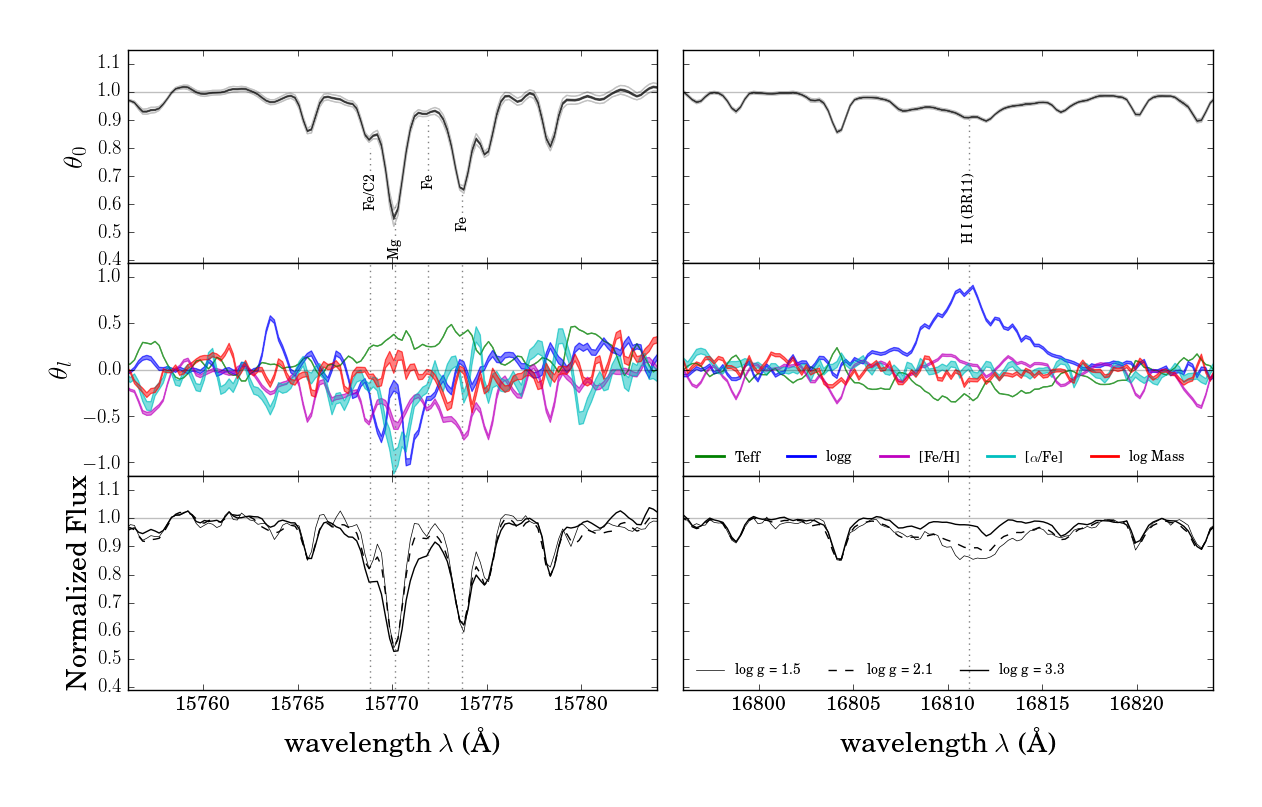
\includegraphics[scale=0.51]{./plots/coeffs_g_3.png}
  \caption{The 0$^{\mbox{th}}$ and first order coefficients ($\theta_0$ , $\theta_{\mbox{ref}}$) of the model trained on the \aspcap\ stars showing the two 30 Angstrom wavelength regions where the \logg\ coefficient (in blue) reaches its highest absolute amplitude. The 0$^{\mbox{th}}$ coefficient (at top) describes the intersect spectrum and relevant spectral absorption features are marked. The middle panel shows all coefficients, each normalised to their highest amplitude, for all \textit{ref} = \teff, \logg, \feh,\alphafe\ and mass coefficients. The bottom panels show the generated spectra from \tc's model to the reference set of stars used for training, for three increasing values of \logg\ that span the range of \logg\ values in the training set.}
\label{fig:logg}
\end{figure}

The bottom panel of Figure  \ref{fig:logg} shows a generated spectrum from \tc's model for a reference set of stellar parameters of a star in the training set. These reference labels are set at \teff = 4710K, \feh = 0.05 and \alphafe = 0.015, for three different \logg\ values of \logg\ = 1.5, \logg\ = 2.1 and \logg\ = 3.3. From the centre left panel of Figure \ref{fig:logg} it is clear that the flux any given pixel can correlate with multiple labels. Typically some coefficients, like \teff\ and \logg\ show an inverse relationship between the label amplitude and the flux.

The location of the highest amplitude \logg\ linear coefficient, which is shown in the top left-hand panel of Figure \ref{fig:logg}, corresponds to a strong  Mg feature in the \apogee\ spectra. Importantly, the highest amplitude of this coefficient corresponds not to the core of the Mg feature, but to the wings, and in particular, most strongly so for the upper wavelength side of the feature. The core of the Mg feature in fact  corresponds to a significantly lesser amplitude of  the coefficient; clearly in the case of \logg,  there is a dramatic reduction in the information content of these pixels in the core of the feature. Note where the \logg\ coefficient decreases from the wings to the core (in blue) the \alphafe\ label (in cyan) increases so that the largest amount of information in this region for the \alphafe\ label is, conversely, from the core of this feature. This Mg feature at 15770.15 Angstroms, is one of the two strongest Mg features (along with the Mg feature at 15753.29 Angstroms) across the \apogee\ H-band spectral region. 

That the strongest coefficient in \logg\ comes from the wings of a strong Mg line in the H-band \apogee\ spectral region is well-aligned with empirical analyses in other, more comprehensively studied wavelength regions. The wings of strong lines are known \logg\ indicators \citep{Gray2008}. Specifically, the wings of Mg lines in the optical wavelength region, which are sensitive to pressure broadening, are used by \citet{F1997} to derive \logg\ for F and G main sequence stars.  

Similarly, Brackett lines (as well as Balmer and Paschen lines)  are sensitive to pressure (Stark) broadening and are therefore excellent tracers of \logg\ in stars. The second highest amplitude coefficient for the first order linear \logg\ coefficient in the \apogee\ spectral region is at the Brackett feature  at $\approx$ 16810 Angstroms, as shown in the right hand panels of Figure \ref{fig:logg}. The  bottom panel of this Figure (at right) shows how significantly the flux varies as a function of \logg\ for this feature. In addition to being second highest in amplitude, the sign of this coefficient for this feature is positive opposite to that  of the wings of the Mg line. As seen in the bottom panel at left, the wings of the Mg feature deepen with increasing \logg, where as for the Brackett feature at right, the spectral profile flattens with increasing \logg, for any given set of stellar \teff, \feh, \alphafe\ and mass parameters, directly demonstrative of the inverse relative relationship between the two features. 


\subsubsection{Spectral dependencies on \teff} 

Figure \ref{fig:teff} shows the same information as for Figure \ref{fig:logg} but for the two highest \teff\ coefficients, centered on $\approx$ 15338 and 15720 Angstroms. The highest \teff\ coefficients correspond to the cores of two Ti lines in the H-band spectra (one of which is blended also with Fe and the other with CN). The temperature coefficient is typically positive in the \apogee\ spectral region, with exceptions, for example at the Brackett feature shown in Figure \ref{fig:logg} (where it is inversely correlated with the \logg\ coefficient). \teff\ is typically strongly anticorrelated with \feh\ and \alphafe, as seen in Figure \ref{fig:teff}. This anticorrelation reflects that in a spectra at a given \feh, as the temperature increases the lines weaken and so the flux decreases, whereas at a given \teff, as the metallicity increases the lines strengthen, and the flux increases. 

As we have a coefficient at \textit{every} wavelength, which we can map to the chemical elements and molecules in the spectra using the \apogee\ linelist, we can interpret the spectral relationship between labels and flux in more detail than for an integrated and typically blended absorption feature itself.  For example, note the asymmetry in the variation of the \teff\ label in the left-hand bottom panel of Figure \ref{fig:teff}: this asymmetry likely reflects the changing ratio of the blends of the absorption features in the training set (in this case, of Ti and Fe). That is, by a generative modeling the spectra at every pixel in the flux, we optimise the potential to characterise and interpret the data, including \textit{within} given absorption features. This  has important applications for stellar astrophysics. Here our aim is simply to motivate that the information in the spectra or regions of highest spectral dependence on the labels, originates from genuinely sensible and plausible elements and molecular features in spectral space.  

% rather than particular absorption features. It is possible to describe this only with  coefficients that are determined at every wavelength in flux. the coefficients at a given flux are sensitive to particular individual elements, which are blended at the spectral resolution of \apogee, but still separated in their central wavelength value. B which can be developed further beyond the demonstrative regions of spectral dependence in labels shown here. and in general, the changing contribution of elements or molecules within that blended feature

% run run -i makeplot_scatter_test18/spectra_step in /Apogee_ages/ o
\begin{figure}[h!]
\centering
 % \includegraphics[scale=0.31]{./plots/validation.png}
    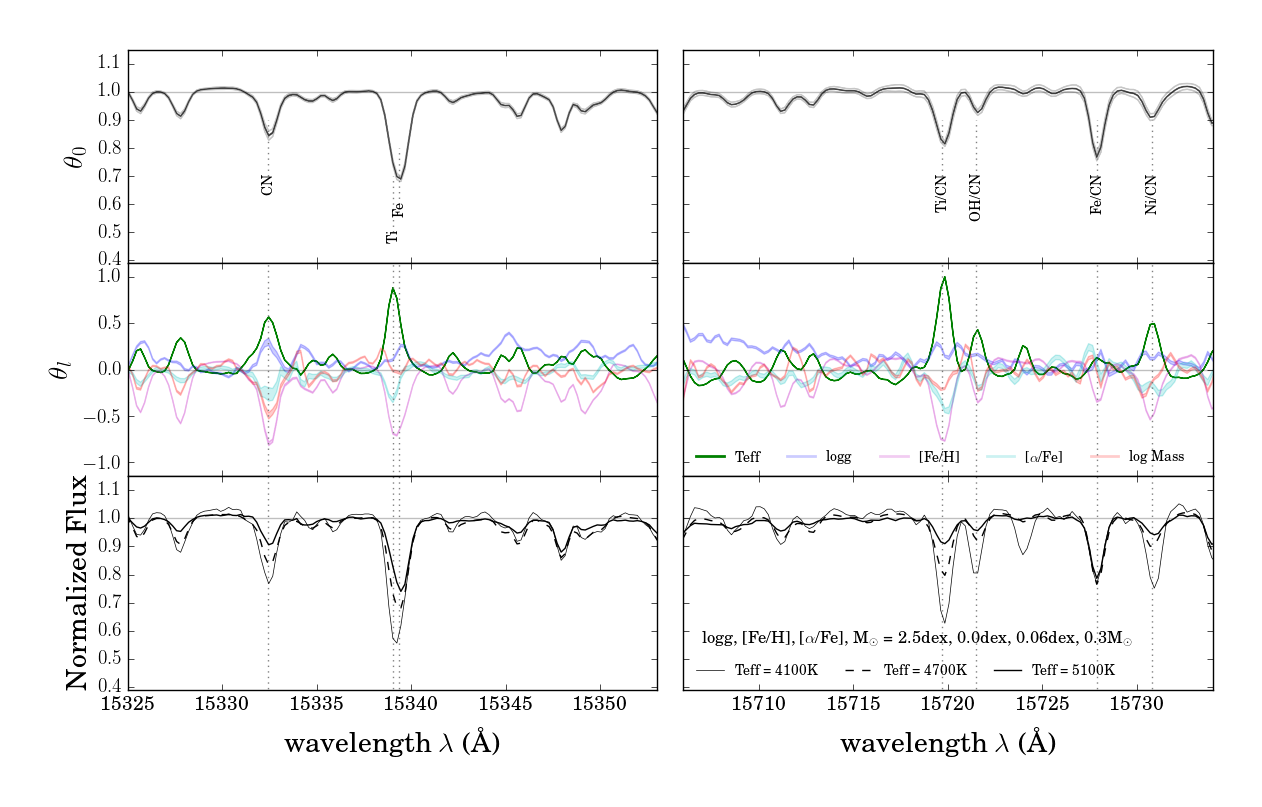
\includegraphics[scale=0.51]{./plots/coeffs_t_3.png}
  \caption{Same as for Figure \ref{fig:logg} but showing the two 30 Angstrom regions centered at the highest \teff\ coefficient (in green).}
\label{fig:teff}
\end{figure}



\subsubsection{Spectral dependencies on \feh\ and \alphafe} 

Figure \ref{fig:feha} is demonstrative of the highest \feh\ and \alphafe\ coefficient in the spectra. The \feh\ and \alphafe\ labels are typically correlated with the cores of all of the absorption features in the spectra, particularly for the \feh\ label, as seen at left. The [M/H] of  a star simply correlates with the \feh\ and the \alphafe\ is known to increase with \feh\ and flattens to a plateau at high \alphafe\ and low \feh, subject to the star formation rate and initial mass function. For many (but not all) absorption features, the \teff\ shows an inverse correlation with temperature as seen in the left hand panel of Figure \ref{fig:teff}. 

The strongest \feh\ coefficient corresponds to a core of a (blended) Mn feature, the flux of which changes dramatically as a function of \feh\ over the range of  --0.8 $<$ \feh\ $<$ +0.2 as shown in the bottom panel of Figure \ref{fig:teff}. Mn is one of the Fe-group elements (in addition to V, Ti, Cr, Co and Ni) and this element is known to correlate directly with \feh\ \citep[see][]{Maria2008, B2015}. 



The largest coefficient in \alphafe\ corresponds to the core of the strong Mg line at $\approx$ 16370 Angstroms (also belnded with CO and OH) and dissimilarly to the \logg\ coefficent, it is the core of the line that correlates with \alphafe. Note that for the \logg\ coefficient at this blended Mg feature in the middle panel of Figure \ref{fig:feha} at right that the \logg\ coefficient is $\approx$ 0 at the very centre of the line profile and increases to a significant dependency in the wings of the feature, primarily for the higher wavelength edge. 


% run run -i makeplot_scatter_test18_step_spectra in /Apogee_ages/ 
\begin{figure}[h!]
\centering
 % \includegraphics[scale=0.31]{./plots/validation.png}
    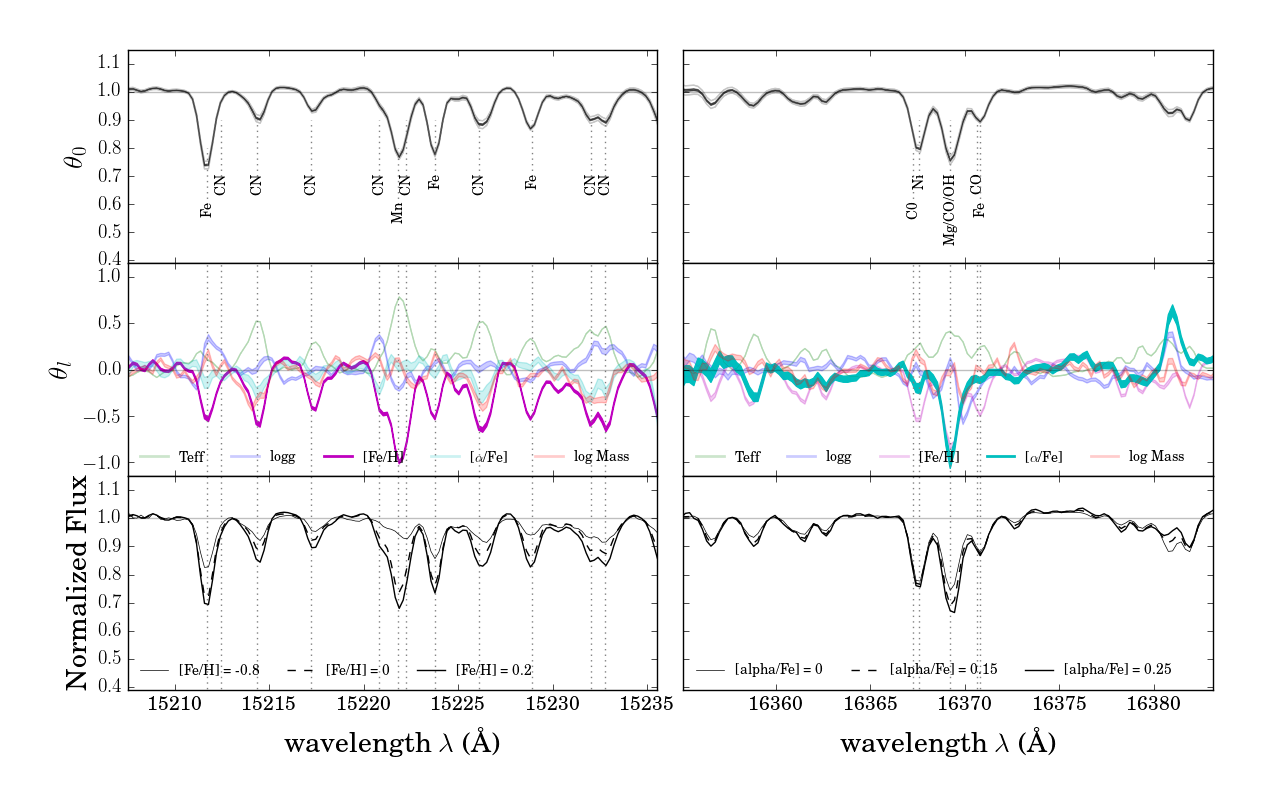
\includegraphics[scale=0.51]{./plots/coeffs_af_3.png}
  \caption{Same as for Figure \ref{fig:logg} but showing the two 30 Angstrom regions centered at the highest \feh\ coefficient (in magenta), at left and highest \alphafe\ coefficient (in cyan), at right.}
\label{fig:feha}
\end{figure}



\subsubsection{Spectral dependencies on mass} 

Finally, having motivated that \tc\ delivers very physically sensible origins of the \teff, \logg, \alphafe\ and \feh\ labels, we examine the origin of the mass information from which we can infer age of \apogee\ stars. 
These first four labels are the least controversial to derive. However, delivering a mass label directly from stellar spectra, particularly given the large stellar surveys like \apogee\ which provide the potential to map ages of stars over a large spatial extent, marks a significant step forward in the exploitation of stellar spectra. With the exception of a few indices which have been used previously to derive mass and inferred age from spectra, this is the first claim of a direct extraction of unique mass information from a stellar spectral region using a general methodology. This approach is not informed by stellar physics. Mathematically this works (as per the cross validation) and now we examine the interpretability of the mass label in chemical elemental abundance space. 

From previous analyses in the UV and optical wavelength regions, we might expect spectral mass indicators, if present, to be realised in (i) chromospheric activity (emission), (ii) drege-up effects (and changing line strengths and profiles of particular elements) or (iii) some combination of individual elemental abundances that reflect the enrichment history of the Milky Way with time (changing element ratios in the spectra). 

Figure \ref{fig:mass} shows the two largest coefficients in the log mass label. The information for the mass label is from (the relatively weak) CN molecular features. Although we show only two regions as demonstrative, we have verified that the five highest mass coefficient amplitudes all correspond uniquely to CN molecular features. The relationship between mass and CN is consistent with the discovery by Martig et al., (2015), in prep., which shows that the [C/N] ratio calculated from \apogee's delivered catalog of C and N abundances in data release DR12 correlates with the mass and inferred age of the \apokasc\ stars. Martig et al., (2015) in prep., use the [C/N] ratio to create a model from these abundances and known masses of the \apokasc\ stars. With \tc\, this information is similarly exploited, only at the spectral level itself: we do not inform \tc's generative model about the origin of the information (instead we rely on stellar physics to interpret the regions where the information is highest). 

From the synthesised spectra in the bottom left-hand panel, it is apparent that it is not only the line strength that changes with the mass coefficient, but rather it is the line profile. Furthermore, from inspection of the second highest mass coefficient at right, it is clear that the spectra changes only very weakly in some locations where the mass coefficient is high. Indeed, the changes in spectra as a function of mass are in general very subtle compared to the other labels. This is likely responsible for the relatively large scatter in the mass label determined with the take-stars out test, shown in Figure 1. Note the other stellar labels have been historically well determined from spectra, even without general mathematical methods like \tc, which optimally exploist all of the available and potential information. The correlations contained in the traditional stellar labels of \teff, \logg, \feh\ and \alphafe\ are more straightforward to extract (e.g. \feh\ correlates with the cores of most absorption features in the spectra). This highlights the strength of an approach like \tc\ to determine and quantify the information that can be truly extracted from data, particularly as a function of signal to noise. 

Examining the CN molecular regions in more detail, the two CN regions shown in Figure \ref{fig:mass} with the highest mass coefficients are in fact a blend of CN molecules containing both $^{12}$C and $^{13}$C. It is this ratio which may drive the changing line profile as a function of mass and may play an important role in delivering the mass information from \apogee\ spectra. This is because the $^{12}$C/$^{13}$C ratio is known as one of the best diagnostics of deep mixing in stellar interiors and so is known to contain information with respect to stellar mass.  In addition to being diagnostics of stellar mass, by being markers of the mixing history of the stars, carbon isotope ratios have also used to differentiate first ascent giants and red clump stars \citep[see][and references therein]{Taut2013}. These elements change abundances during dredge-up, which is effectively the mixing during stellar evolution where by the CN in the hydrogen envelope of a stars interior are bought up to the surface. This happens as the star evolves off the main sequence and up the giant branch \citep{Gilroy1991}. As a consequence of the first dredge up, $^{12}$C decreases whilst $^{13}$C and $^{14}$N show corresponding increases \citep{Taut2010}. 
% and is relatively insensitive to stellar parameters

%With \tc, which exploits the spectral region in full, the information from which the mass is derived from likely includes additional elements to C and N 
%
%and also more regions of CN then \aspcap, which uses a subset of set spectral windows to derive individual C and N abundances. Although the information from \tc\ is then coming from an optimally largest set of flux in the spectra, the information content in any given flux may be very small, even for the highest coefficients. For example, from the bottom right hand panel of Figure \ref{fig:mass} in particular, it is clear that there is only a very marginal change in the spectra as a function of mass. This is dramatically smaller than for the other labels, even for the highest mass coefficient at left. Note there is also a non-linear change in the spectra with linear mass which can be seen by inspection of the flux corresponding to the lowest, intermediate and highest mass spectra generated in the bottom panels. 
%
%The ages can be inferred directly from the spectral mass labels without relying on pipeline measurements of individual abundances, which are known to degrade quickly with decreasing SNR \citep[e.g.][]{Hayden2015}. 


%
% The data-driven model and derivation of mass directly from the spectra itself means that \tc\ will be able to maximally exploit the information in the spectra and as signal to noise decreases, to return masses which can be used to infer ages for \apogee\ stars.  

\begin{figure}[h!]
\centering
 % \includegraphics[scale=0.31]{./plots/validation.png}
    
\includegraphics[scale=0.51]{./plots/coeffs_m_3.png}
  \caption{Same as for Figure \ref{fig:logg} but showing the two 30 Angstrom regions centered at the highest mass coefficients (in red).}
\label{fig:mass}
\end{figure}



%The first dredge up significantly changes the abundances of $^{12}$C and $^{14}$N, decreaseing the carbon by around 30 percent and increasing the nitrogen by 80 percent.  \citep{Taut2013}.

%\tc\ is the ideal tool to extract even fractional and very subtle differences in the spectral flux, which would otherwise be very difficult to determine, using an integrated absorption feature equivalent width measurement alone.





\subsection{The generative model compared to test data}

The \apogee\ sample comprises primarily red giant stars and a subset of  $\approx$ 20,000 red clump stars, identified by \citet{Bovy2014}. We take our model, trained using the reference \apokasc\ stars and determine the stellar parameters and masses for these red clump stars. which cover a radial extent of 6 -- 14 kpc and are located at heights $|z|$ $<$ 1.5 kpc. The red clump sample is a representative and unbiased sample of Milky Way disk stars located across a large radial extent and with an expected age distribution peaking at about 2 Gyr with a tail out to old ages (see Figure X of Bovy et al., 20XX). 


In Figure \ref{fig:spectra}, the spectra of one of the red clump stars, showing a typical red clump spectra, is shown in the black line, for each of the wavelength regions for which the highest amplitude of the coefficients is shown (Figures \ref{fig:logg} -- \ref{fig:mass}).  This star has parameters returned with \tc\ of \teff\ = 4843 K, \logg\ = 2.5 dex, \feh\ = --0.06 dex, \alphafe\ = 0.04 and mass = 1.0 and the interpolated age using the PARSEC isochrones and red clump evolutionary state is 10.6 Gyrs. The data is shown in black, the synthesised spectra from the parameters of \tc\ for this star are in blue and the best fit model from the \apogee\ stellar parameters pipeline \aspcap\ is shown in red. The generated model from \tc\ provides a better fit to the data than the best fit synthetic model from available to \aspcap, demonstrating the 5-labels well describe the flux behaviour of the red clump sample stars the training sample. Note that one of the regions where \aspcap\ performs most poorly is the brackett line which is highly \logg\ sensitive. This may indicate a problem with the model stellar atmospheres or it's associated oscillator strength for this feature. 

%t1,g1,feh1,alpha1,age1, mass1 = 4708.49983734, 2.17652168722, 0.0617198884138, 0.015425129037, 1.55488236009, 1.88141910392

%run -i makeredclumpplot.py
\begin{figure}[h!]
\centering
      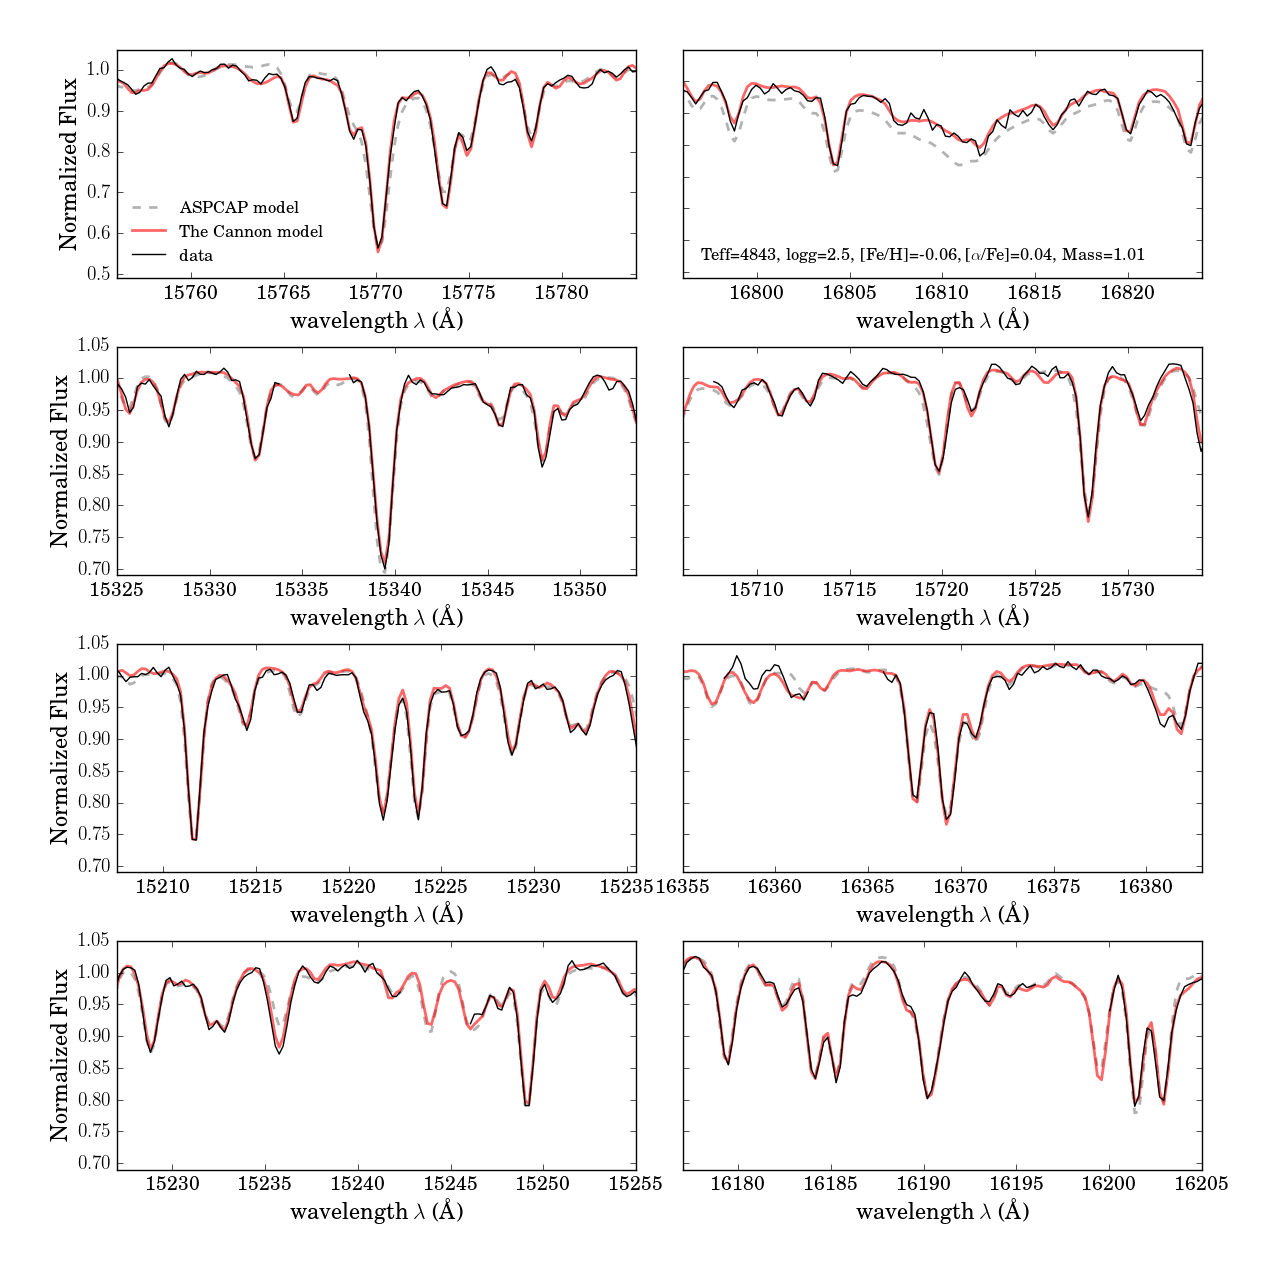
\includegraphics[scale=0.5]{./plots/spectra_fits_7.png}
  \caption{A spectra of one of the red clump stars in the catalogue of \citet{Bovy2014} shown in black, with the best fit model from \tc\ in blue. The best fit model from \aspcap\ is shown in red.}
\label{fig:spectra}
\end{figure}


\section{Discussion}

%We demonstrate the validity of the stellar masses and ages by three
%methods:
%Cross-validation demonstrates that the method obtains (log) mass accuracies of approximately 0.08~dex and (log) age accuracies
%of roughly 0.25~dex for typical-quality \apogee\ spectra.
%Second, we find that the spectral mass (or age) indicators
%discovered by \thecannon\ are associated with elements that can be ``dredged up'',
%specifically the CN regions of the spectra.
%Third, we show that the ages of stellar structures in the
%Milky Way follow gross expectations, even conditioned on abundances.
%All three of these tests show that we can obtain red-giant mass and
%age information from stellar spectra; these capabilities open up new
%opportunities for Milky Way and stellar astrophysics.

We have demonstrated that mathematically, \tc\ works and can return labels of \teff, \logg, \feh, \alphafe\ and mass for \apogee\ spectra. We have shown where the information is contained in the stellar spectrum that most informs each of these labels. Most importantly, that the mass information is derived from weak CN regions, which is a physically sensible origin of the mass dependence given expectations from stellar evolution and changes in these elements from dredge-up mixing processes as the star moves along the red giant branch. We have shown that at test time for the red clump stars, stars that have not been used in training, the model that is generated by \tc's best fit labels provides an excellent match to the real spectra (for stars within the label-range of the training set). In fact, the data-driven model of \tc\ trained on these five labels only (so no individual abundances) provides a better match to the real data than the synthetic stellar models utilised by \aspcap.

With the mass label returned by \tc\ and the inferred age, we are not simply reproducing the \alphafe\ information. We demonstrate this in a number of ways. We examine the age information within small monoabundance boxes in \feh-\alphafe\ space for the training sample and investigate the trends as a function of radius for young and old stars for the low-alpha sequence of the red clump stars as well as the mean age map of the Milky Way disk as traced by the red clump stars.


\subsection{The monoabundance age distribution of the \apokasc\ sample}

In Figure \ref{fig:alphabins} the \apokasc\ training sample is shown in the \alphafe-\feh plane, binned into monoabundance, or small boxes, within this space and the panel at the far left indicates how many stars are in each of these bins. The colormap represents the mean age and the age dispersion from \tc, at left and centre panels respectively. These are the stars used for training and therefore have both the input label on mass (or inferred age) from the seismic scaling relations and the output label on mass and inferred age from \tc. In Figure \ref{fig:mono} a sampling of three of these bins and then all of the bins plotted together is shown, for the individual age label for each star, from \tc\ on the x-axis and from Kepler on the y-axis, minus the mean age value in age monoabundance bin. If there was no additional information in each of the monoabundance bins with respect to age, that is, if the age information was simply a redelivery of the \alphafe\ label then there would be no expected correlation between the difference in \tc\ and Kepler and the mean age. That there is a 1:1 relation between these two axes reflects that \tc\ works mathematically to determine the mass label and that the mass label within a monoabundance bin carries additional information.

% made in makealphamap3.py  in Apogee_ages after running plotdiff_5labels2
% run -i /Users/ness/new_laptop/Apogee_ages/makealphamap4_logmass.py
\begin{figure}[p!]
\centering
 \includegraphics[scale=0.45]{./plots/alpha_feh_bins3.pdf}
    \caption{The \feh-\alphafe\ plane colored by mean age of the stars in each bin. The number of stars in each bin is indicated }
\label{fig:alphabins}
\end{figure}

\begin{figure}[p!]
\centering
 \includegraphics[scale=0.45]{./plots/alpha_feh_std3.pdf}
    \caption{The \feh-\alphafe\ plane colored by standard deviation of the age of the stars in each bin. The number of stars in each bin is indicated }
\label{fig:alphabins}
\end{figure}

% made in makealphamap4_logmass.py after running the plotdiff as above
\begin{figure}[p!]
\centering
 \includegraphics[scale=0.45]{./plots/Kepler_Cannon_diff.pdf}
    \caption{The stars in Figure 8 individually subtracted from the mean age in their respective bin, showing correlation within the individual mono-abundance bins in the \alphafe-\feh\ plane. }
\label{fig:alphabins}
\end{figure}



\subsection{Age maps of the Milky way disk from 6--14 kpc with \apogee\ spectra}

We determine the masses and infer the ages for the $\approx$ 20,000 red clump stars which have distances to approximately 5 percent. The catalogue of ages we provide in Table X for the red clump stars represents the largest homogeneous sample of stars in the Milky Way with associated age labels, and extends the age mapping from the previous local neighborhood only (GCS) to trace the inner to outer disk of the Milky Way, from 6 -- 14 kpc.  

We provide the full age catalog for \apogee's red giant stars, in addition to the red clump stars, adopting the red giant evolutionary state for the transformation from mass label to age label, and provide these data in Table 2, but use only the red clump stars to demonstrate the age trends of the Milky Way disk due to their small distance uncertainties. 


Figure \ref{redclump} shows the mean age of the red clump stars in the \alphafe-\feh plane and the density distribution of these stars (top panels).  We select the low-alpha sequence only to examine the trends of the metallicity \feh\ as a function of radius for the low compared to the intermediate age stars. This selection is for all stars below the dashed line in the density Figure at top right. Presumably, in selection of these stars we are selecting stars along a single sequence of chemical enrichment history and we might expect differences in the distribution of \feh\ as a function of radius for this sequence as a function of age, due to Galaxy evolution processes. The box in the density map is for a small monoabundance population that we select for plotting the trends of inferred age and radius for a small region of chemical homogenity, as additionally demonstrative of the information within the age label, even within a narrow abundance space. 

Examining now the metallicity distribution of the low-alpha sequence with radius, the bottom panels of Figure \ref{fig:redclump} compare the distribution of \feh\ for the XXX stars with ages $<$ 1 Gyrs, at left and the YYY stars with ages $>$ 5 Gyrs, at right. It is clear that the distribution $>$ doubles in width in both the radial direction and with \feh. The relationship between metallicity and radius is weaker for the older stars. Note that the apparent overdensity at about 8kpc across all \feh\ represents the Kepler field in the sample. That the \feh-radius correlation weakens with age likely reflects dynamical evolution processes in the Milky Way, such as radial migration, so that stars within this age range have been redistributed from their birth place, as a scattered weaker trend would imply. The youngest stars have been subject to much lesser dynamical timescales and more tightly traces the origin of their birthplace in the trend seen here between radius and \feh\. The gradient measured for this population from a simple best fit straight line to this distribution at young ages $<$ 1 Gyr is XXX dex/kpc $\pm$ YY kpc. 

\ldots MKN question: Should I fit a model to quantify the 2D age gradient to get median age as a function of (z,R) so we can write down an equation for the age of the red clump as a function of thees params? What form should this take

%in the The dashed line in the right hand panel of this Figure, where the density of the red clump stars is plotted, shows the selection that we have made for analysis of the low-alpha sequence of these stars only. This figure also shows a small box in \feh-\alphafe\ space that we have selected to examine the age trends of the Galaxy over, also demonstrative of the additional information contained within the mass and inferred age label for the true age distribution of stars in the Milky Way (and so in addition to the chemical enrichment marker of \alphafe). 

For the red clump sequence we now show the maps of the median age of the stars across the disk as a function of radius. We show this in Figure \ref{fig:redclump_age} for (i) all stars, at left, (ii) the low alpha sequence, centre and (iii) the mono-abundance sample bin shown in the top right panel of \ref{fig:redclump} at right. These maps show, that even in a homogenous chemical abundance space, ages become younger moving to larger radius, at a given height from the plane, reflecting inside out formation. At a radius, ages also become older moving away in height from the plane and transition to older ages higher from the plane as radius increases. These trends are seen most clearly for all stars, in the left hand panel, the age distributions flare vertically as a function of galactocentric radius. Examining the low-alpha sequence and monoabundance bin within the low alpha sequence in the centre and right hand panel, it is clear that the stars are predominantly young but that the older stare are located furthest from the plane and the height the older stars are located at increases as R increses. Old alpha-poor stars are observed, the low alpha sequence does not represent a homogenous population of young stars, so the \alphafe is not a direct proxy for the age of a star. 

%Could fit a quadratic form for this model: z=ax2+by2+cxy+dx+ey+f. 
%
%Then predict the median age for any star in any region.


%run -i makealphafeh_imshow_3panel.py and readin_ages.py
\begin{figure}[p!]
\centering
 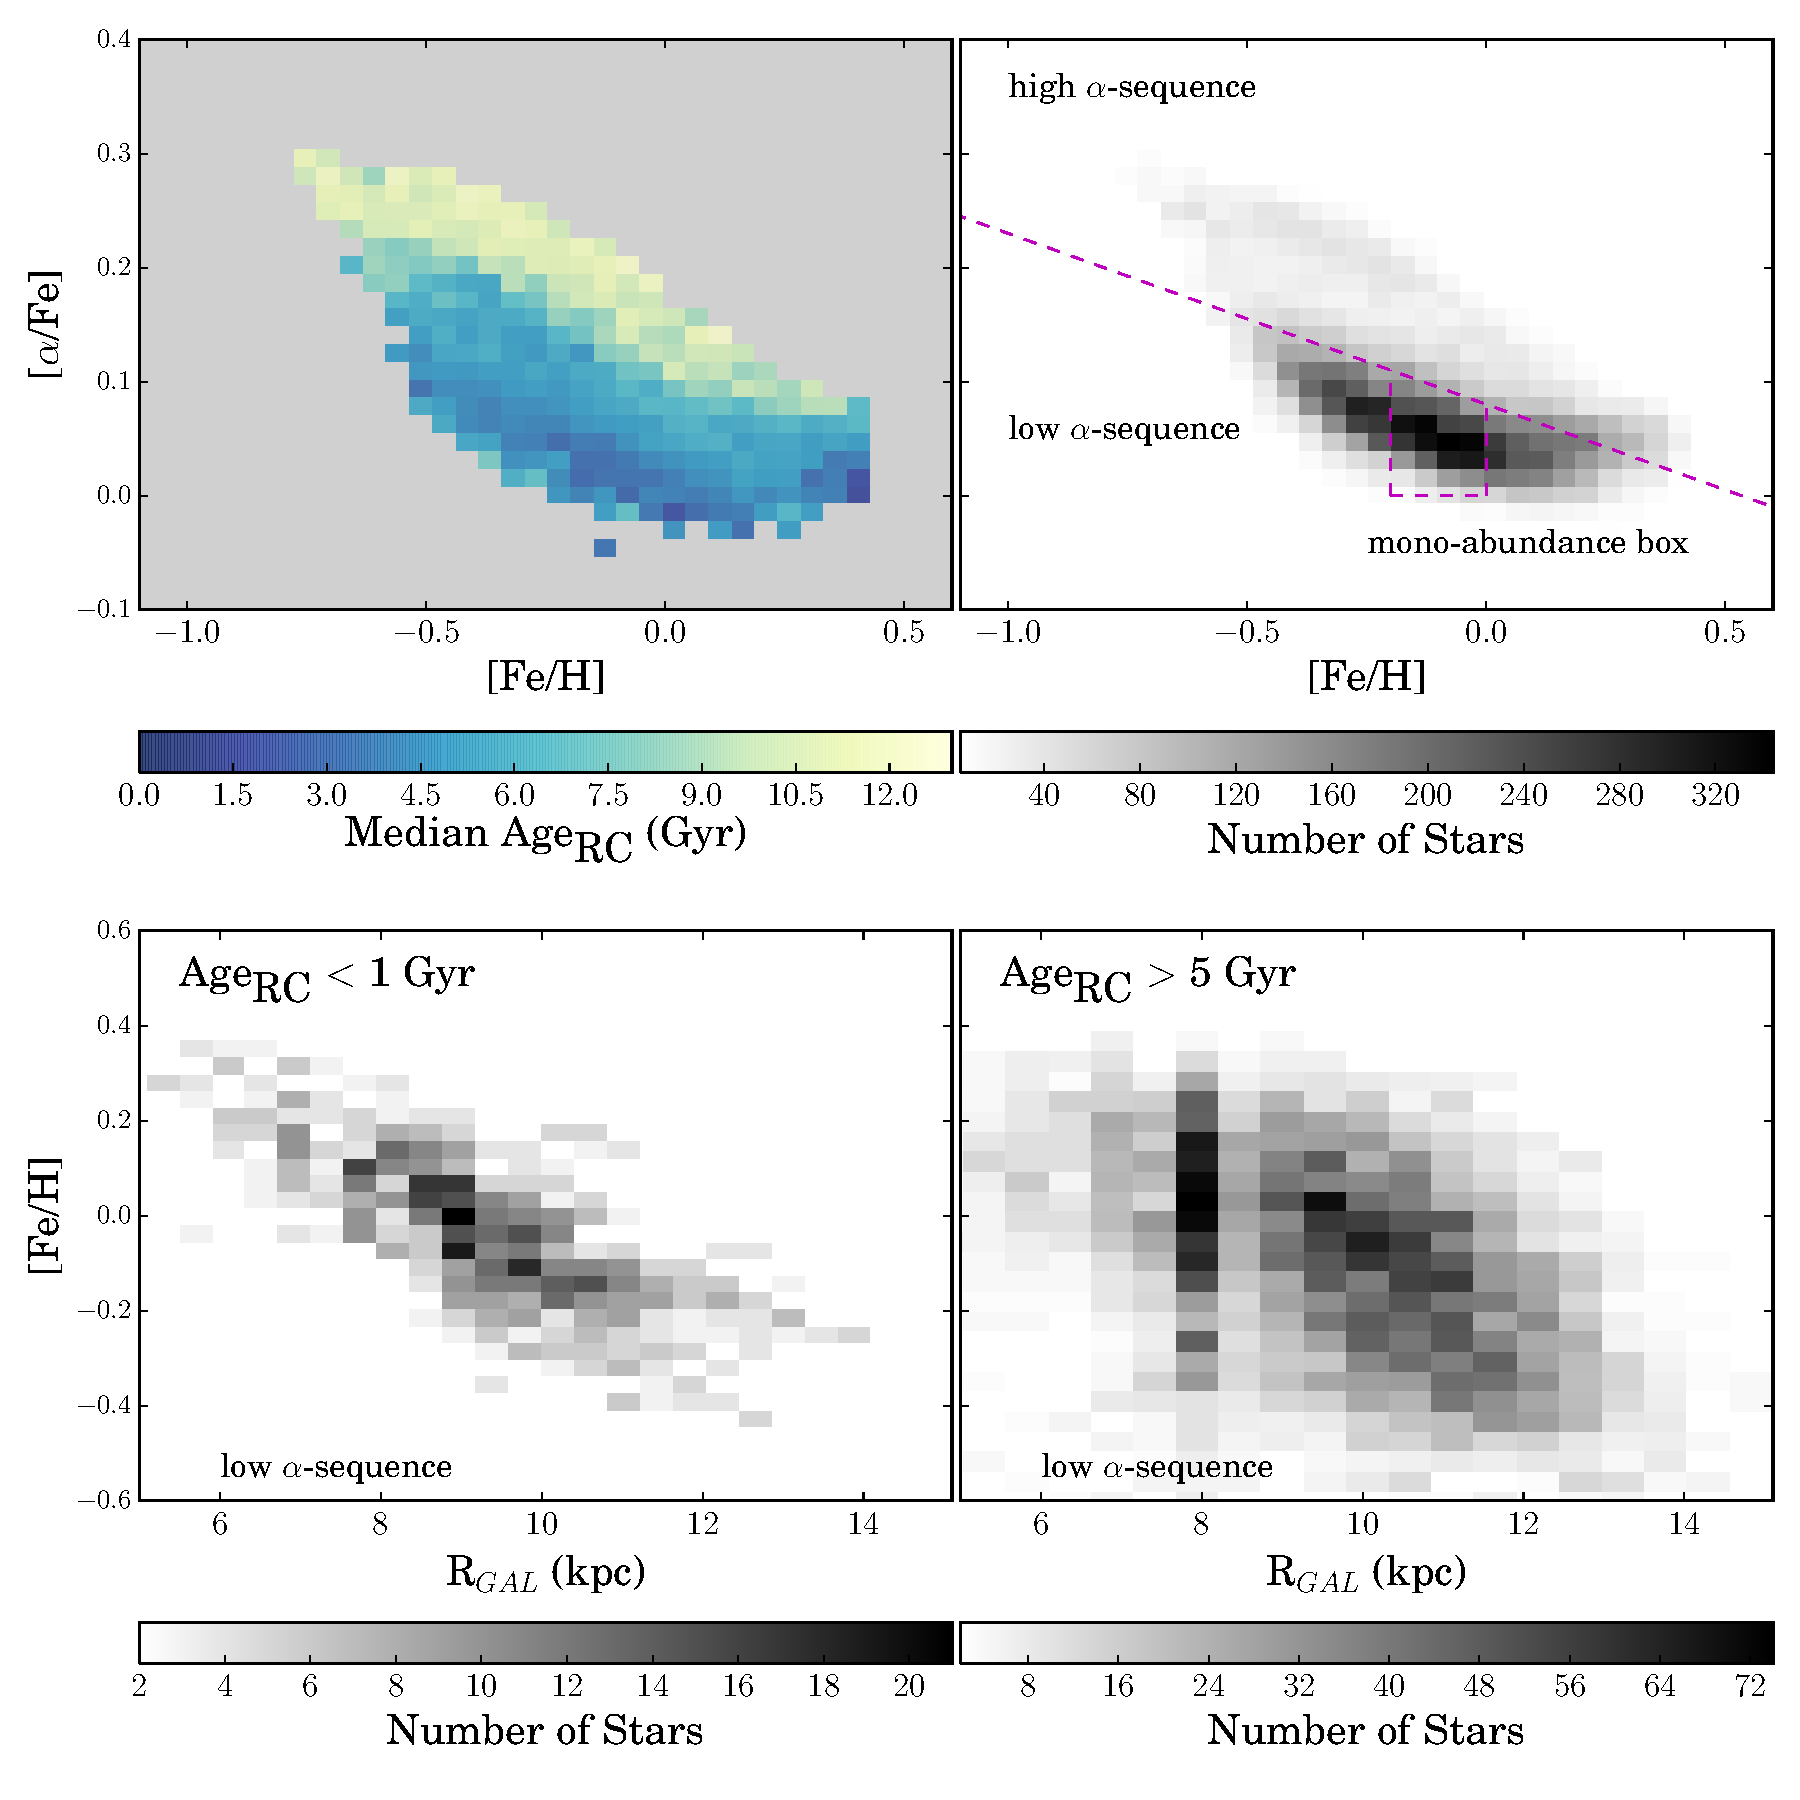
\includegraphics[scale=0.4]{./plots/redclump_4panel.pdf}
    \caption{The 20K red clump sample: low alpha sequence is broken up into radius and box is the mono-abundance distribution in later figure.}
\label{fig:redclump}
\end{figure}

% made in /Users/ness/new_laptop/Apogee_ages/dwh/makeplots_mkn.py 
\begin{figure}[p!]
\centering
 % \includegraphics[scale=0.31]{./plots/validation.png}
    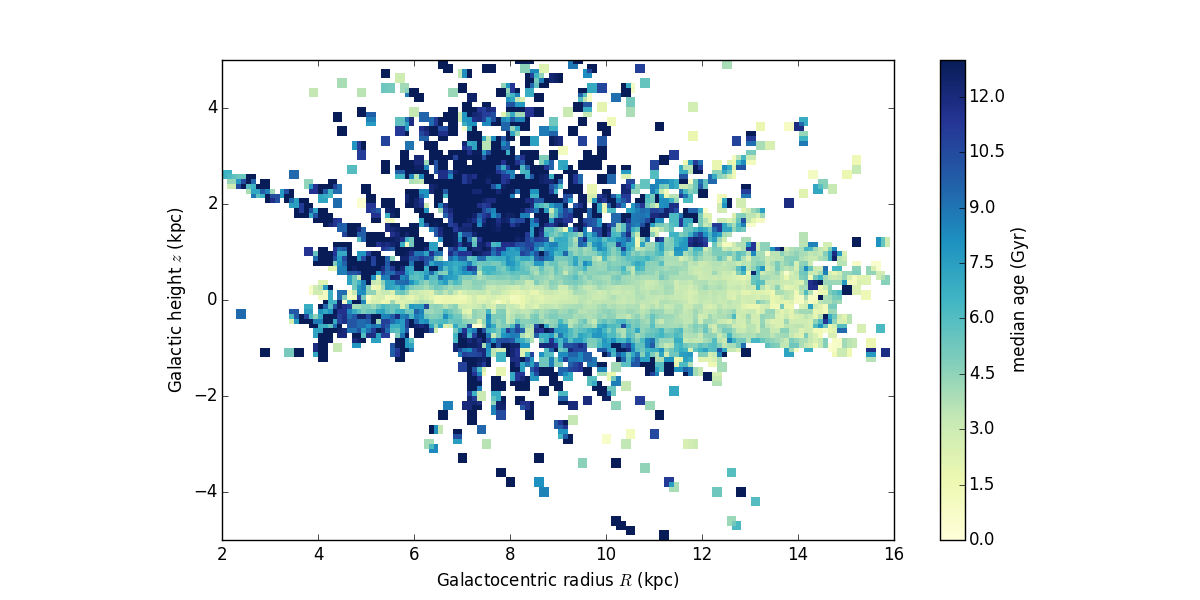
\includegraphics[scale=0.45]{./plots/median_age_abs.png}
    \caption{The median age of the 20,000 red clump stars  }
\label{fig:redclump_age}
\vspace{360pt}
\end{figure}

% made in /Users/ness/new_laptop/Apogee_ages/dwh/makeplots_mkn.py 
\begin{figure}[p!]
\centering
 % \includegraphics[scale=0.31]{./plots/validation.png}
    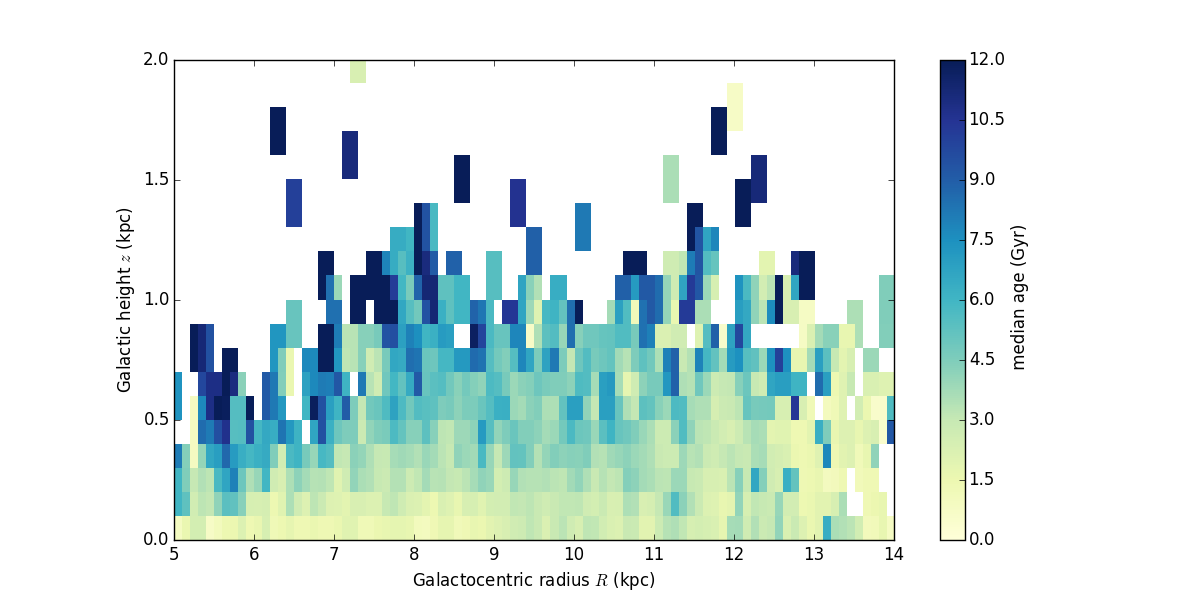
\includegraphics[scale=0.45]{./plots/median_age_low_alpha_abs.png}
    \caption{The median age of the low alpha sequence of the red clump stars ( draw where this in in feh alphafeh plane). Include number of stars. }
\label{fig:redclump_low}
\vspace{-30pt}
\end{figure}


% made in /Users/ness/new_laptop/Apogee_ages/dwh/makeplots_mkn.py 
\begin{figure}[p!]
\centering
 % \includegraphics[scale=0.31]{./plots/validation.png}
    \includegraphics[scale=0.45]{./plots/median_age_mono_abs.png}
    \caption{The median age of low alpha sequence monoabundance  bin with a cut on  \feh\ of 0 to -0.2. }
\label{fig:redclump_mono}
\end{figure}


\subsection{Catalogue}

- put in that have 1's where in extrapolated regime \\
- put in that it is mass that is trained on so the catalogue is coming from that but also have column when trained on ages. \\



%\begin{figure}[p!]
%\centering
% % \includegraphics[scale=0.31]{./plots/validation.png}
%    \includegraphics[scale=0.3]{./plots/median_age_high_alpha_abs.png}
%    \caption{median age of high alpha sequence = draw where this in in feh alphafeh plane. }
%\label{fig:alphabins}
%\end{figure}


\ldots DWH: Re-cap of what we have achieved and how we know we have
succeeded.

\ldots DWH: Emphasis on the reason that the science result is so
convincing that we really have an age indicator here.

\ldots MKN: How do you obtain our code, data, and results?

\section{Conclusion} 



The derivation of stellar masses directly from stellar spectra using \tc\ is highly relevant for other wavelength regions and surveys, like GALAH, (the spectral region of which contains two strong H-$\alpha$ features, already known to be good mass indicators). 

\acknowledgments
It is a pleasure to thank Maria Bergemann (MPIA)
  John Bochanski (Rider),
  Dan Foreman-Mackey (UW), and
insert other relevant people here.
for valuable discussions and contributions.
This project made use of
  The NASA Astrophysics Data System,
  and open-source code in the \project{numpy} and \project{scipy} packages.

[Insert SDSS boilerplate here.]

All code and data produced in this project is available HERE and THERE.

\bibliography{tc.bib}

\end{document}
